% ##################################################################################################################
\chapter{Baoding: A Case Study for Testing a New Household Utility Function in MATSim}
\label{ch:baoding}
\hfill \textbf{Authors:} Chengxiang Zhuge, Chunfu Shao

\editdone{This text has undergone the professional edit. Please no grammatical changes anymore! They are most-probably wrong.}

%\ah{wording? scenario vs. configuration (also in Figures!)} \ah{also in other chapters}

% ##################################################################################################################
\section{Introduction}
Baoding is a medium-sized city in Hebei Province, China. 
The Baoding case study---testing a new household utility function---proposed two scenarios to compare the performance of two utility functions: the household and individual utility function. 
In Scenario~1, it was assumed that each household sought to maximize their overall household utilities when they scheduled; thus, family members' communication and coordination was communal in each household. In Scenario~2, the individual utility function---the default utility function in \gls{matsim}---was utilized to score plans; here, each agent tried only  to maximize his own utilities without communicating with other family members. 

Overall, Scenario~1 differed from Scenario~2 only in the utility function; other input data and parameters in these two scenarios were kept the same. 
The scenarios simulated only urban residents' travel behavior. 
In 2007, the study area population was 1\,060\,783, in 299\,850 households, encompassing 355\,465 privately owned cars.  

% ##################################################################################################################
\section{Population and Demand Generation}
% .................................
\paragraph{Population} The scenarios' agent population was created using a new population synthesis, which  starts with initial household weights obtained from the ~2007 Baoding  Household Travel Survey. 
The final household weights, used for creating the population, were calculated by iteratively adjusting initial household weights in a directed way. 
Gender and household car ownership were also used as person- and household-level control variables, respectively. 
In the scenarios, only 20\,\% of Baoding's total population, approximately 212\,000, was synthesized and used, to speed up the simulation. 

% .................................
\paragraph{Travel Demand Generation}
For initial demand generation, a \gls{ga}, adopting utility maximization theory, was implemented. 
For Scenario~1, this \gls{ga} used the new proposed household utility function as the fitness function; this was employed to generate initial individual daily plans for each household in the synthetic population. 
Specifically, in the \gls{ga}, each chromosome represented a household's set of daily plans and each gene represented a family member's daily plan. 
During evolution (including mutation, crossover and selection), each chromosome was scored; only those with higher household utilities remained. 
Then, a set of daily plans with the highest household utility function were selected and allocated to the household. 
Similarly, other daily household plans in the synthetic population were generated, one by one. 
It should also be noted that the travel time in the initial daily plans was estimated. 
Therefore, elements like travel time and activity duration in the initial daily plans would be adapted (optimized) when executed in \gls{matsim}.

In Scenario~2, the \gls{ga} incorporated the individual utility function to search for each agent's (family member's) plans.

% ##################################################################################################################
\section{Activity Locations, Network and Transport Modes}
% .................................
\paragraph{Activity Locations} Five typical activity types, including work, home, leisure, education and shopping, were taken into account in the scenarios. 
The activity facilities numbers for these five types were: 1647, 462, 246, 372 and 445, respectively. 

% .................................
\paragraph{Transport Network} The scenarios contained two network types, including road and public transit networks. 
Figure~\ref{fig:baoding_fig1} demonstrated Baoding's~2007 road and transit network. The road network was composed of 1\,650 nodes and 539 links; the transit network contained transit routes and transit schedules, with  49\,transit lines and (98\,transit routes). 

% .................................
\paragraph{Transport Modes} The simulated transport modes included car, public transport, bike and walk. Car drivers and public transport passengers used the road network and transit network. Because agents who traveled by bike or on foot had no access to the transport network, they were teleported from origin to destination and assigned no exact routes, but their travel time was calculated. 

% ##################################################################################################################
\section{Historical Validation}
Historic validation. composed of the following two steps, was carried out to assess \gls{matsim}'s performance and applied to both scenarios. 

Step~1: Comparison of both real and simulated car flows and comparison of real and simulated transit passenger flows were carried out in each scenario, to assess  \gls{matsim}'s performance for car and transit simulation. 
The \gls{mre},  calculated by the equation~(\ref{eq:baoding_mre}), was employed to assess performance.

\begin{equation}
\label{eq:baoding_mre}
MRE = \frac{\lVert F_{simulated} - F_{real} \lVert}{F_{real}} \times 100\,\%
\end{equation} 
where, $F_{simulated}$ and $F_{real}$ denotes the simulated and the real flow (car flow or passenger flow), respectively.

Step~2: Comparison of both scenarios' performance for car and transit simulation, based on results from step~1. 

% ===========================================================================
\subsection{Comparison of Two Scenarios: Car Traffic}
Car flow data on six road links (equal to 12\,links in \gls{matsim} scenario) from 7\,am to 9\,am, was used for comparison of car simulation and was manually counted in~2007. 

Figure~\ref{fig:baoding_fig2a} demonstrated car simulation performance for both scenarios. 
Four dots were approximately located in the $y=x$ line and the other two dots, below the line, also were very close to it. 
Mean relative error margins of Scenario~1 and Scenario~2 were 44.8\,\% and 47.5\,\%, respectively. 
I can thus be concluded that the performance of Scenario~1 (using  household utility function) was slightly better than Scenario~2 (using individual utility function). 

% ===========================================================================
\subsection{Comparison of Two Scenarios: Transit Traffic}
Data (passenger flow for nine transit lines from 7\,am to 9\,am) used for transit simulation comparison was also manually counted in 2007. Figure~\ref{fig:baoding_fig2b} illustrated both transit simulation scenarios' performance. 
Clearly, most dots did locate close to the $y=x$ line, however, two dots below the line were significantly distant from it. 
Also, mean relative errors of Scenario~1 and Scenario~2 were 38.7\,\% and 47.9\,\%, suggesting 
that Scenario~1 better represented transit passenger flows than Scenario~2. 

% ##################################################################################################################
\section{Achieved Results}
A proposed \gls{matsim} household utility function was tested comparing two scenarios using household and individual utility function. Historical validation confirmed that \gls{matsim} improved its own car and transit simulation performance by using the new utility function. 
However, more case studies are needed to further confirm this new proposed utility function's advantages.

% ##################################################################################################################
More information on the Baoding scenario can be found in \citet[][]{Zhuge_PhDThesis_2014} (in Chinese) 

 % ------------
\createfigure%
{Road and transit network of Baoding in~2007}%
{Road and transit network of Baoding in~2007}%
{\label{fig:baoding_fig1}}%
{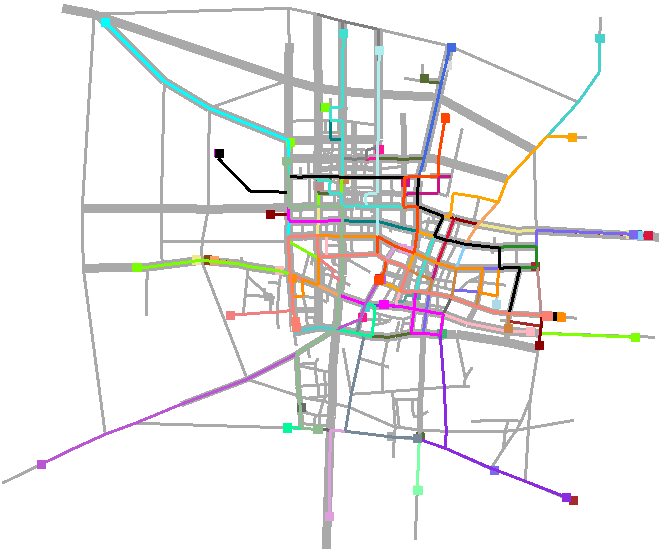
\includegraphics[width=0.8\textwidth, angle=0]{scenarios/figures/baoding_fig1.png}}%
{}
% ------------

% ------------
\createfigure%
{Performance comparison of Scenario~1 and~2}%
{Performance comparison of Scenario~1 and~2}%
{\label{fig:baoding_fig2}}%
{%
  \createsubfigure%
  {Car}%
  {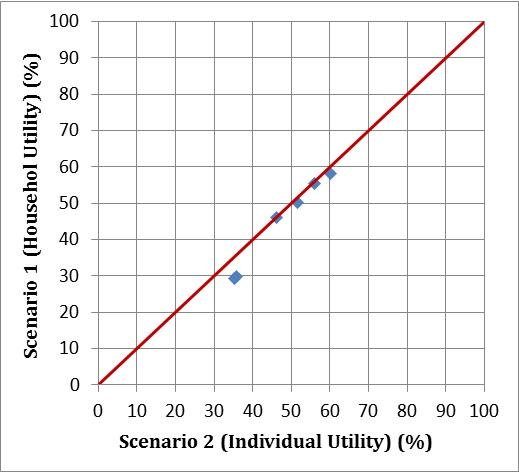
\includegraphics[width=0.7\textwidth,angle=0]{scenarios/figures/baoding_fig2a.png}}%
  {\label{fig:baoding_fig2a}}%
  {}%
  \createsubfigure%
  {Public transit}%
	{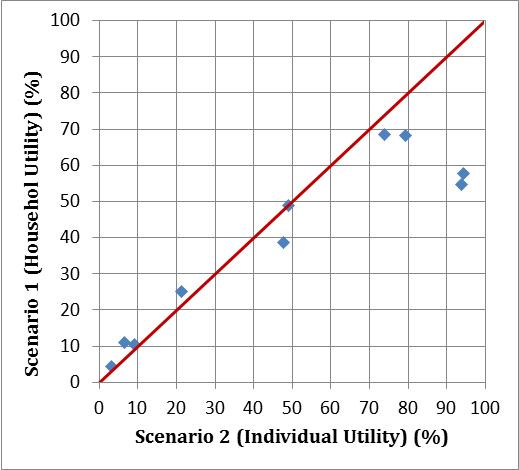
\includegraphics[width=0.7\textwidth,angle=0]{scenarios/figures/baoding_fig2b.png}}%
  {\label{fig:baoding_fig2b}}%
  {}%
}%
{}
% ------------

% ##################################################################################################################
